\documentclass{standalone}
\usepackage{tikz}
\usetikzlibrary{arrows,positioning}
\begin{document}

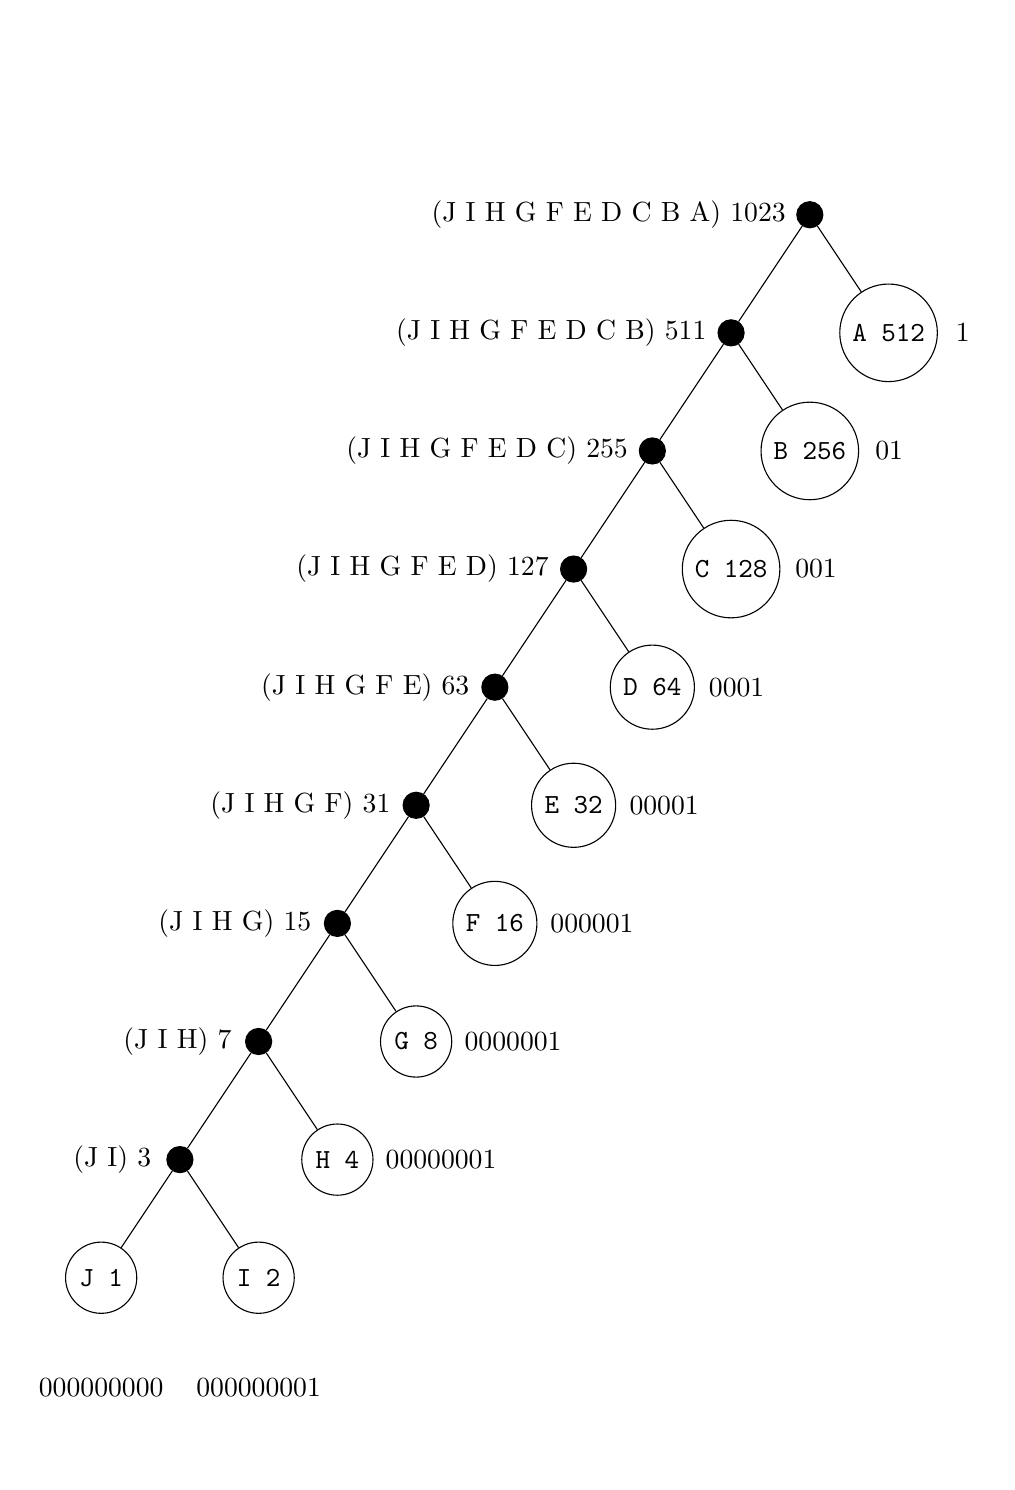
\begin{tikzpicture} [
	level 1/.style = {sibling distance=20mm},
	every node/.style = {draw, circle, fill=black},
	leaf/.style = {draw, circle, minimum size = 5mm, fill=none}
]
\node [label=left:(J I H G F E D C B A) 1023] {}
	child {node [label=left:(J I H G F E D C B) 511] {}
		child {node [label=left:(J I H G F E D C) 255] {}
			child {node [label=left:(J I H G F E D) 127] {}
				child {node [label=left:(J I H G F E) 63] {}
					child {node [label=left:(J I H G F) 31] {}
						child {node [label=left:(J I H G) 15] {}
							child {node [label=left:(J I H) 7] {}
								child {node [label=left:(J I) 3] {}
									child {node [leaf] [label=below:000000000] {\texttt{J 1}}}
									child {node [leaf] [label=below:000000001] {\texttt{I 2}}}}
								child {node [leaf] [label=right:00000001] {\texttt{H 4}}}}
							child {node [leaf] [label=right:0000001] {\texttt{G 8}}}}
						child {node [leaf] [label=right:000001] {\texttt{F 16}}}}
					child {node [leaf] [label=right:00001] {\texttt{E 32}}}}
				child {node [leaf] [label=right:0001] {\texttt{D 64}}}}
			child {node [leaf] [label=right:001] {\texttt{C 128}}}}
		child {node [leaf] [label=right:01] {\texttt{B 256}}}}
	child {node [leaf] [label=right:1] {\texttt{A 512}}};
\end{tikzpicture}

\end{document}
